Más especificamente, \textcolor{red}{estimamos un RTT promedio} para cada salto que se da en
la ruta que nos comunica con cada host, y \textcolor{red}{normalizamos este valor para
conseguir un ZRTT} para cada salto que nos de suficiente informaci\'on como para
\textcolor{red}{analizar el trasfondo del tr\'afico en la red}.

\begin{figure}[!h]
  \begin{center}
      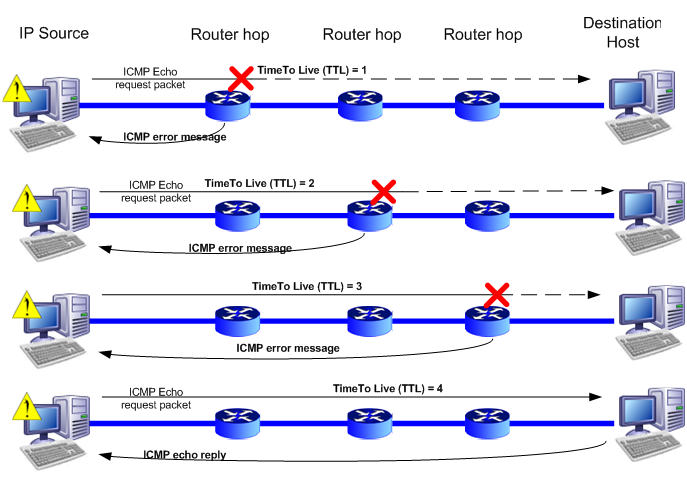
\includegraphics[scale=0.4]{imagenes/traceroute.png}
      \caption{Mecanismo de acción de traceroute}
      \label{fig:contra1}
  \end{center}
\end{figure}
